% !TeX spellcheck = en_US
\documentclass{report}
\usepackage{paccosp}
	\makeindex
\begin{document}
	\title{Stochastic Processes notes}
	\author{Kotatsu}
	\date{\small vaffanculo}
	\maketitle
	\pagenumbering{Roman}
	\begin{preface}
Let's have a fucking party!
		
		\vskip1.2cm
		
		\hfill Kotatsu
	\end{preface}
	\clearpage
	\tableofcontents
	\pagenumbering{arabic}
\chapter{Brownian Motion}	
	\section{Continuity of stochastic processes}
	The sample path in a discrete scenario is given by
	\begin{equation*}
		\pr(X(t)<x|\F_{s})=\pr(X(t)<x|X_{s}).
	\end{equation*}
	This gives us a sample path like this:
	\begin{figure}[H]
		\centering
		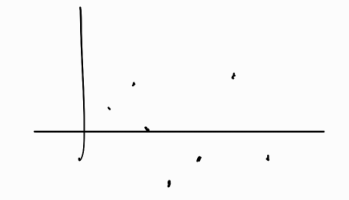
\includegraphics[width=0.7\linewidth]{img/screenshot003}
		\caption{Fucking hell.}
		\label{fig:screenshot003}
	\end{figure}
	We want to think, though, about a continuous space and time process: 
	\begin{figure}[H]
		\centering
		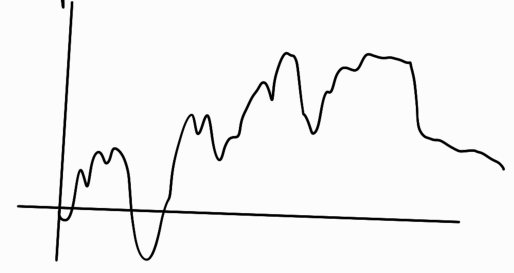
\includegraphics[width=0.7\linewidth]{img/screenshot004}
		\caption{Leaning like my academic career.}
		\label{fig:screenshot004}
	\end{figure}
	How can we define the continuity of the sample paths? and how can we check this property? There are some possible definitions of continuity. To control for their robustness we check whether according to each of these definitions the Poisson process, a discrete process, is correctly classified as non continuous.
	\begin{definition}
		A stochastic process $\{M(t)\}$ is said to be a \emph{counting process} if:
		\begin{enumerate}[i.]
			\item $M(t)>0$;
			\item $M(t)$ is an integer;
			\item $M(t)$ is increasing, meaning that $s\leq t\implies M(s)\leq M(t)$.
		\end{enumerate}
	\end{definition}
	In general, these processes count how many times an event happens.
	\begin{definition}
		A Poisson process is a counting process such that:
		\begin{enumerate}
			\item $N(0)=0$;
			\item for $t_1<t_2<t_3<t_4$ we have
			\begin{equation*}
				N(t_2)-N(t_1)\independent N(t_4)-N(t_3)
			\end{equation*}
			meaning that the increments are independent;
			\item for $\every h>0$ and $t>\tau$ it holds:
			\begin{equation*}
				N(t)-N(\tau)\sim N(t+h)-N(\tau+h)
			\end{equation*}
			meaning that the increments are stationary (the origin start doesn't matter);
			\item we have $$\pr(N(t)=k)=\frac{(\lambda t)^{k}}{k!}e^{-\lambda t}\qquad\text{for } k=0,1,\ldots$$
		\end{enumerate}
	\end{definition}
	\begin{figure}[h]
		\centering
		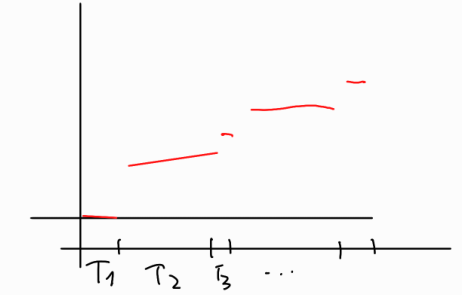
\includegraphics[width=0.7\linewidth]{img/screenshot002}
		\caption{I am very good at drawing straight lines.}
		\label{fig:screenshot002}
	\end{figure}
	
	The inter-arrival times are i.i.d. \rv s distributed as
	\begin{equation*}
		T_i\distexp{\lambda}.
	\end{equation*}
	The continuity of sample paths can be characterized in four different ways:
	\begin{enumerate}
		\item \emph{Continuity in mean squares}: we have this if for $\every t\geq0$ we have
		\begin{equation*}
			\lim_{s\to t}\ev\left[|X(t)-X(s)|^{2}\right]=0.
		\end{equation*}
		So according to this definition, the mean square of the distance goes to 0 if we go near $s$.
		\item \emph{Continuity in probability}: we have this if for $\every t\geq0$ and $\every\varepsilon>0$ we have
		\begin{equation*}
			\lim_{s\to t}\pr(|X(t)-X(s)|>\varepsilon)=0.
		\end{equation*}
		This should be enough for all finite distributions, right?\footnote{First, but not last, question without an answer.}
		\begin{theorem}
			Let $\{X(t)\}$ be a stochastic process such that $\ev[X^{2}(t)]<\infty$ for all $t$. Then it is continuous in mean squares\ifonly{}:
			\begin{enumerate}
				\item $m(t)=\ev[X(t)]$ is continuous;
				\item the covariance function
				\begin{equation*}
					\Gamma(s,t)=\ev[(X(t)-m(t))(X(s)-m(s))]
				\end{equation*}
				is continuous on its diagonal set.
			\end{enumerate}
			\begin{fancyproof}
				Consider the expectation
				\begin{equation*}
					\ev\left[|X(t)-X(s)|^{2}\right]=\ev\left[|X^{2}(s)+X^{2}(t)-2X(t)X(s)|\right]\tag{\faAdjust}\label{boh}
				\end{equation*}
				but
				\begin{equation*}
					\ev\left[X^{2}(s)\right]=\ubracketthin{\ev\left[(X(s)-m(s))^{2}\right]}_{\Gamma(s,s)}+2m(s)\ev\left[X(s)\right]-m^{2}(s)
				\end{equation*}
				and
				\begin{equation*}
					\ev\left[X^{2}(t)\right]=\Gamma(t,t)+2m(t)\ev[X(t)]-m^{2}(t)
				\end{equation*}
				and, moreover,
				\begin{equation*}
					\ev[X(s)X(t)]=\Gamma(s,t)-\cancel{m(t)m(s)}+m(t)\ev[X(s)]+\cancel{m(s)\ev[X(t)]}.
				\end{equation*}
				So \ref{boh} becomes
				\begin{align*}
					\text{\faAdjust}&=\Gamma(s,s)+2m^{2}(s)-m^{2}(s)+\Gamma(t,t)+2m^{2}(t)-m^{2}(t)-2\ev\left[X(s)X(t)\right]\\
					&=\Gamma(s,s)+\Gamma(t,t)-2\Gamma(s,t)+m^{2}(t)+m^{2}(s)-2m(t)m(s)\\
					&=\Gamma(s,s)+\Gamma(t,t)-2\Gamma(s,t)+\left[m(t)-m(s)\right]^{2}.
				\end{align*}
				Hence, if $m(t)$ is continuous and $\Gamma(s,t)$ is continuous for $s=t$ then the process is continuous because we have:
				\begin{itemize}
					\item $[m(t)-m(s)]^{2}\to0$ since it is a continuous function;
					\item $\Gamma(s,s)+\Gamma(t,t)-2\Gamma(s,t)$ that becomes $\Gamma(t,t)+\Gamma(t,t)-2\Gamma(t,t)=0$.
				\end{itemize}
				I'd like to add that dear prof. Sacerdote didn't explain this last little point. Thank you! So now whe have
				\begin{equation*}
					\ev\left[|X(s)-X(t)|^{2}\right]\to0.
				\end{equation*}
				If this holds for $m(t)$ and $\Gamma(t,t)$ then it is continuous in mean squares.
			\end{fancyproof}
		\end{theorem}
		\begin{remark}
			A process continuous in mean \faSquare[regular] (get it?) is continuous in probability (use Chebyshev\footnote{Like use him? As a person? He is dead.}).
		\end{remark}
		Is the Poisson process continuous in mean \faSquare[regular] (and also in probability)? We know that
		\begin{equation*}
			m(t)=\lambda t
		\end{equation*}
		and 
		\begin{align*}
			\Gamma(s,t)&=\ev[(N(t)-m(t))(N(s)-m(s))]\\
			&=\ev[N(t)N(s)]-2m(t)m(s)-m(t)m(s)\\
			&\underset{t>s}{=}\ev[(N(t)-2N(s)+N(s))N(s)]-m(t)m(s)\\
			&=\ev[(N(t)-N(s))N(s)]+\ev\left[N^{2}(s)\right]-m(t)m(s)\\
			&=\ubracketthin{\ev[N(t)-N(s)]}_{
			\lambda(t-s)}\ubracketthin{\ev(N(s))}_{\lambda s}+\ev\left[N^{2}(s)\right]-\ubracketthin{m(t)}_{\lambda t}\ubracketthin{m(s)}_{\lambda s}\\
			&=\lambda^{2}(\cancel{t}-s)s-\cancel{\lambda^{2}ts}+\ev\left[N^{2}(s)\right]\\
			&=-\lambda^{2}s^{2}+\ubracketthin{\var N(s)}_{\lambda s}+\ubracketthin{\left[\ev\left[N(s)\right]\right]^{2}}_{\lambda^{2}s^{2}}\\
			&=\lambda s\qquad\text{if }s<t.
		\end{align*}
	\begin{figure}[h]
		\centering
		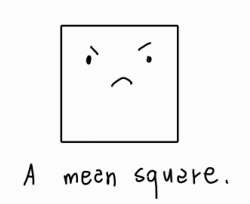
\includegraphics[width=0.3\linewidth]{img/screenshot001}
		\caption{Sei un fallito.}
		\label{fig:screenshot001}
	\end{figure}
	So $\Gamma(s,t)=\lambda\min(s,t)$ is continuous on diagonal and $m(t)=\lambda t$ is also continuous... but this would mean that Poisson processes are continuous! Which they shouldn't be! Do I care? No!
	\item \emph{Almost sure continuity}: we can ask, as a requirement, that
	\begin{equation*}
		\pr\left(\lim_{s\to t}N(s)=N(t)\right)=1.
	\end{equation*}
	Does this finally solve the problem with the Poisson processes? No, because it verifies the almost sure continuity (since it is discontinuous only in a countable number of instances).\\
	It is not enought ot think point by point: we must think \textit{uniformly}.
	\begin{definition}
		A stochastic process $\{X(t)\}$ has almost sure continuous sample paths if, with probability 1, $X(t)$ is a continuous function, that is:
		\begin{equation*}
			\pr(X(t)\text{ has continuous samples})=1.
		\end{equation*}
	\end{definition}
	Of course, the case in which you have exceptional points is not a problem since they have measure 0.
	\begin{figure}[h]
		\centering
		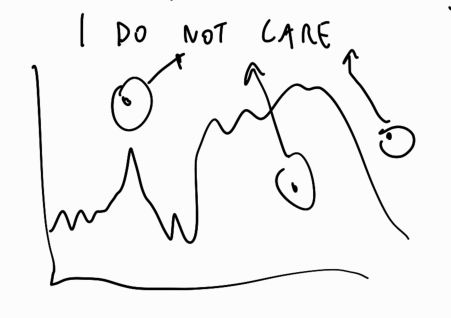
\includegraphics[width=0.4\linewidth]{img/screenshot005}
		\caption{Me neither.}
		\label{fig:screenshot005}
	\end{figure}
	\begin{remark}
		The set
		\begin{equation*}
			\{\omega\in\Omega:t\to B_{t}(\omega)\text{ is continuous}\}
		\end{equation*}
		is not necessarily in the \sa{} generated by the vectors
		\begin{equation*}
			\left(B_{t_{1}}, B_{t_{2}},\ldots,B_{t_{n}}\right)\qquad n\in\N.
		\end{equation*}
	\end{remark}
\end{enumerate}
\section{Definitions of Brownian motion}
\subsection{Historical context}
Imagine a spherical particle with a diameter of $10^{-6}$ m surrounded by $10^{-23}$ (the Avogadro number) molecules with a diameter of $10^{-10}$ m of diameter.
\begin{figure}[h]
	\centering
	\begin{tikzpicture}
		\shade[ball color = gray!40, opacity = 0.4] (0,0) circle (1.2cm);
		\draw (0,0) circle (1.2cm);
		\draw (-1.2,0) arc (180:360:1.2 and 0.6);
		\draw[dashed] (1.2,0) arc (0:180:1.2 and 0.6);
		\fill[fill=black] (0,0) circle (1pt);
		\draw[dashed] (0,0 ) -- node[above]{\tiny$10^{-6}\;m$} (1.2,0);
		\foreach \a in {1,2,...,17}{
			\draw (\a*360/17: 2cm) circle (0.2cm);
			\shade[ball color=Green3,opacity=0.6] (\a*360/17: 2cm) circle (0.2cm);
		}
	\end{tikzpicture}
	\caption{My balls.}
	\label{fig:screenshot006}
\end{figure}
How can we model the behavior of this ball in a mathematical way\footnote{At this point of the lesson Prof. Sacerdote started ranting about Machine Learning (seriously?) being a black box for like 10 minutes.}?\\
In 1828 Robert Brown (fig. \ref{fig:autecre}) observed the chaotic movement of pollen in the water through a microscope and noted:
\begin{itemize}
	\item the motion was composed by translations and rotations;
	\item particles seemed to move independently one from the other;
	\item smallest particles moved more actively;
	\item less viscous fluids determined more activity movement;
	\item the motion never ceased;
	\item the motion was not determined by liquid flows or evaporation;
	\item particles were not animated.
\end{itemize}
In 1905 Einstein gave the correct explanation formulating a model that also proved valid for forecasting: the idea was that the atoms surrounding the particles (the atoms of the fluid) performed a temperature-dependent movement that collided with the particles, changing their direction.\\
\begin{figure}[h]
	\centering
	
\includegraphics[width=0.5\linewidth]{img/screenshot006}
	\caption{Autechre are a IDM duo from Rochdale, England, composed by Robert Brown and Sean Booth.}
	\label{fig:autecre}
\end{figure}
In 1906 the Polish mathematician Smoluchowski independently obtained results similar to Einstein's. Unrelated, but in 1909 Jean Perrin determined the size of atoms.\\
The Einstein approach considers the motion of a particle over a small interval $T$ observed in a time large enough to see at least 2 intervals $t$ independent. Consider, for the sake of simplicity, the one-dimensional case. During $t$ the particle moves of a distance $\Delta$, that is a \rv{} with density $\varphi(\Delta)$ that must be symmetric so $\varphi(\Delta)=\varphi(-\Delta)$. For example, we can imagine $\varphi(\Delta)\sim\mathsf{N}$ with mean 0 (since in this model we do not expect a drift) and small variance. Then we can consider
\begin{equation*}
	\gamma=f(x,t)\qquad\text{as the number of particles per unit of volume.}
\end{equation*}
Einstein proved that $f$ verifies
\begin{equation*}
	\frac{\partial f}{\partial t}=D\frac{\partial^{2}f}{\partial x^{2}}.
\end{equation*}
This was the equation of heat diffusion that was already well known at the time. And so was its solution, which is
\begin{equation*}
	f(x,t)=\frac{1}{\sqrt{4\pi Dt}}e^{-\frac{x^{2}}{4Dt}}.
\end{equation*}
In this case $D$ had a physical meaning: Einstein proved\par
\noindent
\begin{minipage}{0.5\textwidth}
	\begin{equation*}
		D=\frac{1}{\sqrt{6\pi r\eta}}\frac{RT}{N}
	\end{equation*}
\end{minipage}\begin{minipage}{0.5\textwidth}
\begin{itemize}
	\item $\eta$: dynamic viscosity
	\item $r$: dimension of particles
	\item $R$: gas constant (8.3 $\frac{\mathrm{J}}{\mathrm{mol~K}}$)
	\item $T$: absolute temperature
	\item $N$: Avogadro's number
\end{itemize}
\end{minipage}
He could, moreover, calculate the average displacement of a particle
\begin{equation*}
	\lambda_{x}=\sqrt{\overline{x}^{2}}=\sqrt{2Dt}.
\end{equation*}
This means that the displacement (space) is proportional to the square root of time... But what is this story of space and time being related non linearly? This sounded pretty wild for that time.
\begin{figure}[h]
	\centering
	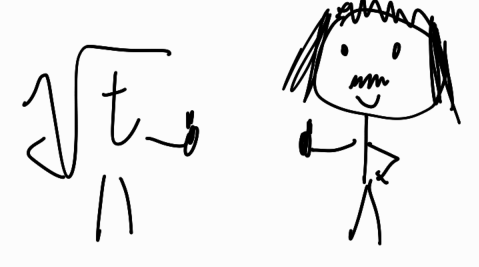
\includegraphics[width=0.5\linewidth]{img/screenshot007}
	\caption{Idk I think I would have probably killed myself.}
	\label{fig:screenshot007}
\end{figure}
\subsection{Random walk model}
We can think that:
\begin{itemize}
	\item each particle starts at $x=0$;
	\item the particle changes position at discrete times
	\begin{equation*}
		k\Delta t \qquad k=1,2,\ldots\qquad\Delta t>0;
	\end{equation*}
	\item the particles move $\Delta x$ units to the right (or to the left) with probability $p=\unmezz$;
	\item $\Delta x$ does not depend on any past position nor on the current position. 
\end{itemize}
\begin{figure}[h]
	\centering
	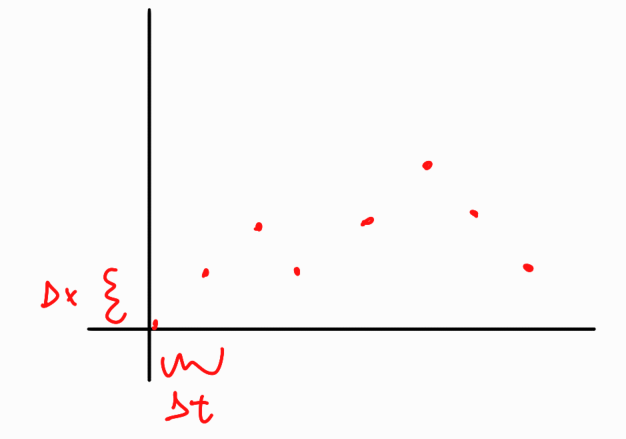
\includegraphics[width=0.5\linewidth]{img/screenshot008}
	\caption{I do not know how to do curly brackets}
	\label{fig:screenshot008}
\end{figure}
When $\Delta x$ and $\Delta t$ go to 0 in an appropriate way, we don't see ``jumps'' anymore but a continuous process:
\begin{figure}[h]
	\centering
	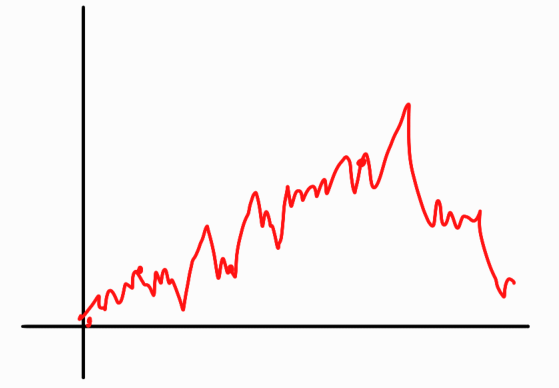
\includegraphics[width=0.5\linewidth]{img/screenshot009}
	\caption{I miss tikzes but they take so much time.}
	\label{fig:screenshot009}
\end{figure}
So we get a continuous process ${\{X_{t}\}}_{t\geq0}$ that is the random position of the time $t$. Introduce the i.i.d. \rv s $\{\varepsilon_{i}\}$ such that $\pr(\varepsilon_{i}=1)=\pr(\varepsilon_{i}=0)=\unmezz$. Then $S_{N}=\sum_{i}^{N}\varepsilon_{i}$ is the number of moves to the right (since moves to the left do not contribute to this count). In the same way, I have $N-S_{N}$ being the number of moves to the left. Now we can write
\begin{align*}
	X_{T}&=\text{positions of particles at }T=N\Delta t\\
	&=S_{N}\Delta x-(N-S_{N})\Delta x\\
	&=(2S_{N}-N)\Delta x\\
	&=\sum_{k=1}^{N}(2\varepsilon_{k}-1)\Delta x.
\end{align*}
\begin{remark}
	For any two times $t=n\Delta t$ and $T=N\Delta t$, $0<t<T$, we can write:
	\begin{align*}
		X_{T}&=(X_{T}-X_{t})+(X_{t}-X_{0})\\
		&=\sum_{k=n+1}^{N}(2\varepsilon_{k}-1)\Delta x+\sum_{k=1}^{n}(2\varepsilon_{k}-1)\Delta x.
	\end{align*}
		\begin{center}
			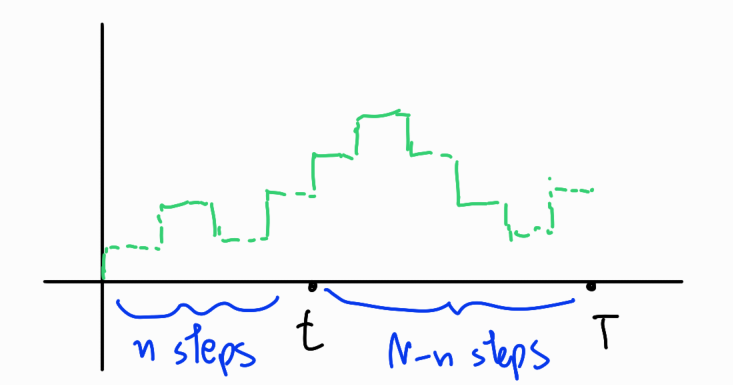
\includegraphics[width=0.5\linewidth]{img/screenshot010}
		\end{center}
	But these quantities involve different $\varepsilon$, so they are independent:
	\begin{equation*}
		X_{T}-X_{t}\independent X_{t}-X_{0}\qquad\text{(independent increments.)}
	\end{equation*}
	But we know that 
	\begin{equation*}
		\ev\varepsilon_{i}=\unmezz\qquad\mathrm{and}\qquad\var\varepsilon_{i}=\frac{1}{4}
	\end{equation*}
	so
	\begin{align*}
		\var X_{T}&=\var\left[\sum^{}{N}_{k}(2\varepsilon_{k}-1)\Delta x\right]\\
		&\overset{i.i.d.}{=}\sum^{N}_{k}\left(\Delta x\right)^{2}\var(2\varepsilon_{k}-1)\\
		&=\sum_{k}^{N}(\Delta x)^{2}\cancel{4}\ubracketthin{\cancel{\var \varepsilon_{k}}}_{\frac{1}{4}}\\
		&=N(\Delta x)^{2}.
	\end{align*}
	But $N=\frac{T}{\Delta t}$ so 
	\begin{equation*}
		N(\Delta x)^{2}=\frac{(\Delta x)^{2}}{\Delta t}T=\sigma^{2}T.
	\end{equation*}
\end{remark}
So this should be the variance of our random walk. If we take the limit for $x$ and $t$ and do nost take into account that space and time decrease in different ways we get a process that has mean 0 and variance 0... but that is a process that is 0 almost surely! So we get the idea that time and space must decrease at different speeds. We also said that the increments must be stationary, but that has its implications.
\begin{remark}
	We know that $\var 2S_{N}=N$, but
	\begin{align*}
		X_{T}&=(2S_{N}-\ubracketthin{N}_{\mathclap{\ev 2 S_{N}}})\Delta x\\
		&=\frac{2 S_{N}-\ev 2 S_{N}}{\mathcolor{Green4}{\sqrt{N}}}\mathcolor{Green4}{\sqrt{N}}\Delta x\\
		&=\frac{2S_{N}-\ev 2 S_{N}}{\sqrt{\var(2S_{N})}}\ubracketthin{\sqrt{N}}_{\sqrt{\frac{T}{\delta t}}}\ubracketthin{\Delta x}_{{\sigma\sqrt{\Delta t}}}\\
		&=\frac{2S_{N}-\ev 2 S_{N}}{\ubracketthin{\sqrt{\var(2S_{N})}}_{\claptext{This gets to $Z\distnorm{0,1}$ as $N\to\infty$}}}\sigma\sqrt{T}.
	\end{align*}
	So we get that this quantity gets to $Z\sigma\sqrt{t}$ and it is true for each $t$:
	\begin{equation*}
		X_{t}\distnorm{0,t\sigma^{2}}.
	\end{equation*}
\end{remark}
\subsection{Definitions}
\begin{definition}
	\emph{Definition of Brownian Motion} (1923, by Norbert Wiener).\\
	A stochastic process $B={\{B_{t}\}}_{t\geq 0}$ defined on a probability space $(\Omega,\F,\pr)$ and taking values in $\R$ is called \emph{standard Brownian motion} (or \emph{standard Wiener process}) if:
	\begin{enumerate}
		\item the function $t\mapsto B_{t}$ is \ul{continuous} from $\R_{+}$ to $\R$ and $B_{0}=0$ (both almost surely);
		\item $B$ has \ul{stationary increments} (they don't depend on the origin):
		\begin{equation*}
			B_{t}-B_{s}\sim B_{t+h}-B_{s+h}\qquad\every 0<s<t\qquad\every f>0;
		\end{equation*}
		\item $B$ has \ul{independent} increments, i.e. for any $0\leq t_{0}\leq t_{1}<\leq t_{2}\leq\ldots\leq t_{n}$ and $n\geq 1$ we have:
		\begin{equation*}
			B_{t_1}-B_{t_0}, B_{t_2}-B_{t_1},\ldots,B_{t_{n}}-B_{t_{n-1}}\qquad\text{independent};
		\end{equation*}
		\item $B_{t}\distnorm{0,t}$ for $\every t\geq 0$.
	\end{enumerate}
\end{definition}
\begin{definition}
	\emph{General Brownian motion} (Brownian motion with drift).\\
	\begin{equation*}
		X_{t}=\ubracketthin{\mu}_{\claptext{drift}} t+\ubracketthin{\sigma}_{D=\frac{\sigma^{2}}{2}} B_{t}.
	\end{equation*}
	This process verifies properties 1, 2, 3 and
	\begin{equation*}
		X_{t}\distnorm{\mu t,\sigma^{2}t}.
	\end{equation*}
\end{definition}
We can now proceed to define the $d$-dimensional \bwm{}:
\begin{definition}
	A $d$-dimensional \bwm, $B={\{B_{t}\}}_{t\geq 0}$ is a stochastic process indexed by $[0,\infty)$ taking values on $\R^{d}$ such that:
	\begin{enumerate}
		\item $B_{0}(\omega)=0$ \as{} $\every\omega\in\Omega$;
		\item $B_{t_{n}}-B_{t_{n-1}},\ldots,B_{t_{1}}-B_{t_{0}}$ are independent fo $\every n>1,\;0\leq t_{1},t_{2}<\ldots<t_{n}<\infty$ (\emph{independent increments});
		\item $B_{t}-B_{s}\sim B_{t+h}-B_{s+h}$ for $\every h>0$, $\every 0\leq s<t<\infty$ (\emph{stationary increments});
		\item $B_{t}-B_{s}\distnorm{0,t-s}^{\otimes d}$ with 
		\begin{equation*}
			\mathsf{N}(0,t)\dx =\frac{\dx}{\sqrt{2\pi t}}\exp\left\{-\frac{x^{2}}{2t}\right\}
		\end{equation*} (\emph{Gaussian increments});
		\item $t\mapsto B_{t}(\omega)$ is continuous for all $\omega$ (\emph{continuity of sample paths}).
	\end{enumerate}
\end{definition}
Remember that 
\begin{equation*}
	1,2,3,5\implies 4\qquad\text{and}\qquad1,2,3,4\implies 5
\end{equation*}
for almost all $\omega$. A standard \bwm{} on $\R^{d}$ is obtained by setting
\begin{equation*}
	B=(B^{1},B^{2},\ldots,B^{d})
\end{equation*}
where $B^{1},B^{2},\ldots$ are independent \bwm{} on $\R$ called \ul{coordinate processes}.
\begin{definition}
	The continuous process $W$ is called \emph{Wiener process} with respect to $\mathscr{A}$ if it is adapted to $\mathscr{A}$ (check that adaptness is included in the above definitions!) and 
	\begin{equation*}
		\ev_{s}f[W_{s+t}-W_{s}]=\int_{\R}\dx\left[\frac{e^{-\frac{x^{2}}{4t}}}{\sqrt{2\pi t}}f(x)\right]\qquad\text{for $f$ positive Borel function and }\every s,t\in\R_{+}.
	\end{equation*}
\end{definition}
\begin{exercise}
	Prove that the second definition of \bwm{} implies the first for $d=1$.
\end{exercise}
But with these properties there is the risk that no such object exists! For example, if we add differentiability to our list of requests then no object satisfies such properties. So we need to ask two questions:
\begin{itemize}
	\item Does \bwm{} exists?
	\item Is it unique?
\end{itemize}
Wiener worked on the difference space, that is the space of the increments of the process, and introduced a Fourier series representation:
\begin{equation*}
	W_t=\xi_{0}t+\sqrt{2}\sum_{n=1}^{\infty}\xi_{n}\frac{\sin(n\pi t)}{\pi n}\qquad0\leq t\leq 1
\end{equation*}
where $\{\xi_{i}\}$ are i.i.d. \rv s $\xi_{i}\distnorm{0,1}$, so this object is a Fourier series for which the coefficients are \rv s. Thinking about difference equations makes our life a bit easier, since different times have different $\xi_{i}$ but these are independent so also the increment between times are independent.
\section{Gaussian processes}
\begin{definition}
	A \emph{Gaussian process} is defined as a process $\Gamma$ with
	\begin{equation*}
		\begin{array}{rclr}
			\frac{\dif}{\dif \lambda}\ev\left[e^{i\lambda\Gamma}\right]\Big|_{\lambda=0}&=&im&m=\ev[\Gamma]\\
			\frac{\dif^{2}}{\dif\lambda^{2}}\ev\left[e^{i\lambda\Gamma}\right]\Big|_{\lambda 0}&=&-\ev\left[\Gamma^{2}\right].&
		\end{array}
	\end{equation*}
\end{definition}
\begin{definition}
	A random vector
	\begin{equation*}
		\Gamma=(\Gamma_{1},\Gamma_{2},\ldots,\Gamma_{n})\in\R^{n}
	\end{equation*}
	is Gaussian if the scalar product 
	\begin{equation*}
		\langle\lambda,\Gamma\rangle\qquad\every\lambda\in\R^{n}
	\end{equation*}
	is a one-dimensional Gaussian \rv{} with:
	\begin{equation*}
		\ev\left[e^{i\langle\lambda,\Gamma\rangle}\right]=e^{i\ev\left[\langle\lambda,\Gamma\rangle\right]-\unmezz\var\left(\langle\lambda,\Gamma\rangle\right)}.
	\end{equation*}
\end{definition}
So setting 
\begin{equation*}
	\begin{array}{cc}
		m=(m_{1},\ldots,m_{n})\in\R^{n}&m_{j}=\ev[\Gamma_{j}]\\
		&\\
		\Sigma={(\sigma_{jk})}_{jk}\in\R^{n\times m}&\begin{array}{rl}
			\sigma_{jk}&=\ev\left[(\Gamma_{j}-m_{j})(\Gamma_{k}-m_{k})\right]\\
			&=\cov(\Gamma_{j},\Gamma_{k})\\
			&=\Sigma_{j,k}
		\end{array}
	\end{array}
\end{equation*}
So that 
\begin{equation*}
	\ev\left[e^{i\langle\lambda,\Gamma\rangle}\right]=e^{i\langle\lambda,m\rangle-\unmezz	\langle\lambda,\Sigma\lambda\rangle}.
\end{equation*}
The basic idea is that I can linearly transform a random vector and it still is a Gaussian \rv. Fourier transform always exists even for limits, while it is not so easy for distributions. What happens if we apply to a Gaussian vector a matrix that turns it into a subspace? Do I care? Not much! But imagine the classic Gaussian \rv:
\begin{equation*}
	f(x)=\frac{1}{\sqrt{2\pi \sigma^{2}}}\exp\left\{-\frac{x^{2}}{2\sigma^{2}}\right\}.
\end{equation*}
If I take $\sigma\to0$ then the density degenerates into a Dirac measure.
\begin{figure}[h]
	\centering
	\begin{tikzpicture}
	\begin{axis}[every axis plot post/.append style={
			mark=none,domain=-2:2,samples=20,smooth}, % All plots: from -2:2, 50 samples, smooth, no marks
		axis x line*=bottom, % no box around the plot, only x and y axis
		axis y line*=left,
		axis lines=center, % the * suppresses the arrow tips
		enlargelimits] % extend the axes a bit to the right and top
		\addplot[SpringGreen3] {gauss(0,0.5)} node[pos=0.75,anchor=south west]{$\sigma_{2}$};
		\addplot[Turquoise4] {gauss(0,0.75)} node[pos=0.9,anchor=south west]{$\sigma_{1}$};
		\addplot[OliveDrab4] {gauss(0,0.2)} node[pos=0.6,anchor=south west]{$\sigma_{3}$};
	\end{axis}
	\end{tikzpicture}
	\label{fig:gaugau}
	\caption{It will become a dirac measure... but that is not a fucking density.}
\end{figure}
This is still technically a measure because it integrates to 1, but it is not a density anymore since we lose dimensionality on $\R$ which is\footnote{As I learn now.} the meaning of becoming a subspace! But now consider the characteristic function
\begin{equation*}
	\ev\left[e^{i\lambda x}\right]=e^{-1\lambda\frac{\sigma^{2}}{2}}\xrightarrow{\sigma\to0}\ubracketthin{1}_{\claptext{characteristic function of degenerate \rv s.}}.
\end{equation*}
The main point about this is that we could still take a limit. If we were working with density we couldn't have done that.\par
The alternative definition for Gaussian processes are:
\begin{definition}
	A vector valued \rv{} $X$ has $n$-dimensional standard Gaussian distribution if its $n$ coordinates are standard Gaussian in $\R^{1}$ and are independent.
\end{definition} 
\begin{definition}
	A vector valued \rv $Y:\Omega\to\R^{n}$ is Gaussian if there exists a vector valued $X$ having $n$-dimensional standard Gaussian distribution and $m\times n$ matrix $A$ and a $m$-dimensional vector $b$ such that
	\begin{equation*}
		Y=AX+b\qquad\text{and }AA^{\trsp}=\Sigma.
	\end{equation*}
\end{definition}
In this case $Y$ us a linear transformation of the Gaussian vector and $A$ projects $X$ in a $m$-dimensional subspace. This is the same procedure we do with Principal Component Analysis, where we diagonalize a matrix and other passages I don't remember and I don't care about.
There are some properties:
\begin{proposition}
	\begin{itemize}
		\item Let $X\distnorm{0,\Sigma_{n}}$. The distribution of $\left[X_{k+1,\ldots,k+n}\right]$ conditioned to $\left[X_{1}=x_{1},\ldots,X_{k}=x_{k}\right]$ is \begin{equation*}
		W(0,\Sigma_{2|1})
		\end{equation*}
		where 
		\begin{equation*}
			\Sigma_{2|1}=\Sigma_{22}-\Sigma_{21}\Sigma_{11}^{-1}\Sigma_{12}
		\end{equation*}
		and 
		\begin{equation*}
			\Sigma=\begin{bmatrix}
				\Sigma_{11}&\Sigma_{12}\\
				\Sigma_{21}&\Sigma_{22}
			\end{bmatrix}.
		\end{equation*}
		Note that the sub-matrices that $\Sigma$ is made of have lower dimensionality.
		\item If $Y=\ubracketthin{a}_{\in\R^{m}}+\ubracketthin{B}_{\in\R^{n}\times\R^{m}}X$ is an affine transformation of $X\distnorm{\mu,\varepsilon}$ then $$Y\distnorm{a+B\mu, B\Sigma B^{\trsp}}.$$
		This is like working with the affine transformation.
	\end{itemize}
\end{proposition}
What about another definition? I think we need it
\begin{definition}
	A Gaussian process is a stochastic process such that for every $t_{1},\ldots,t_{k}$ in the index set $\T$ and each $k>1$ we have that
	\begin{equation*}
		\left(X_{t_{1}},\ldots,X_{t_{k}}\right)=X_{t_{1},\ldots,t_{k}}
	\end{equation*}
	is a multivariate Gaussian random vector (possibly degenerate).
\end{definition}
Now we have defined a class of processes:
\begin{figure}[h]
	\centering
	\begin{tikzpicture}[framed]
		\draw[thick] (0,0) circle (1.5cm) node[anchor=east] {Gaussian processes}
		(2,0) circle (1.5cm) node[anchor=west] {Markov processes} (1,-1.5) circle (1.5cm) node[anchor=north] {Martingle tools};
		\node[anchor=south,yshift=-2.3cm] at (current bounding box.north) {$BM$};
	\end{tikzpicture}
\end{figure}
There is another class: the Levy processes: they have independent and stationary increment (so they are Markov processes) but unlike \bwm{} we don't require continuity on the sample path, but just \ul{continuity on the right of sample paths} and \ul{admit left limit}.
\clearpage
\listoffigures  
\end{document} 


%THIS IS THE DARK AGE OF LOVE   